\section{Datenbanken}\label{sec:Datenbank}
\begin{wrapfigure}{r}{0.5\textwidth}
    \vspace{-1.2cm}
    \begin{center}
      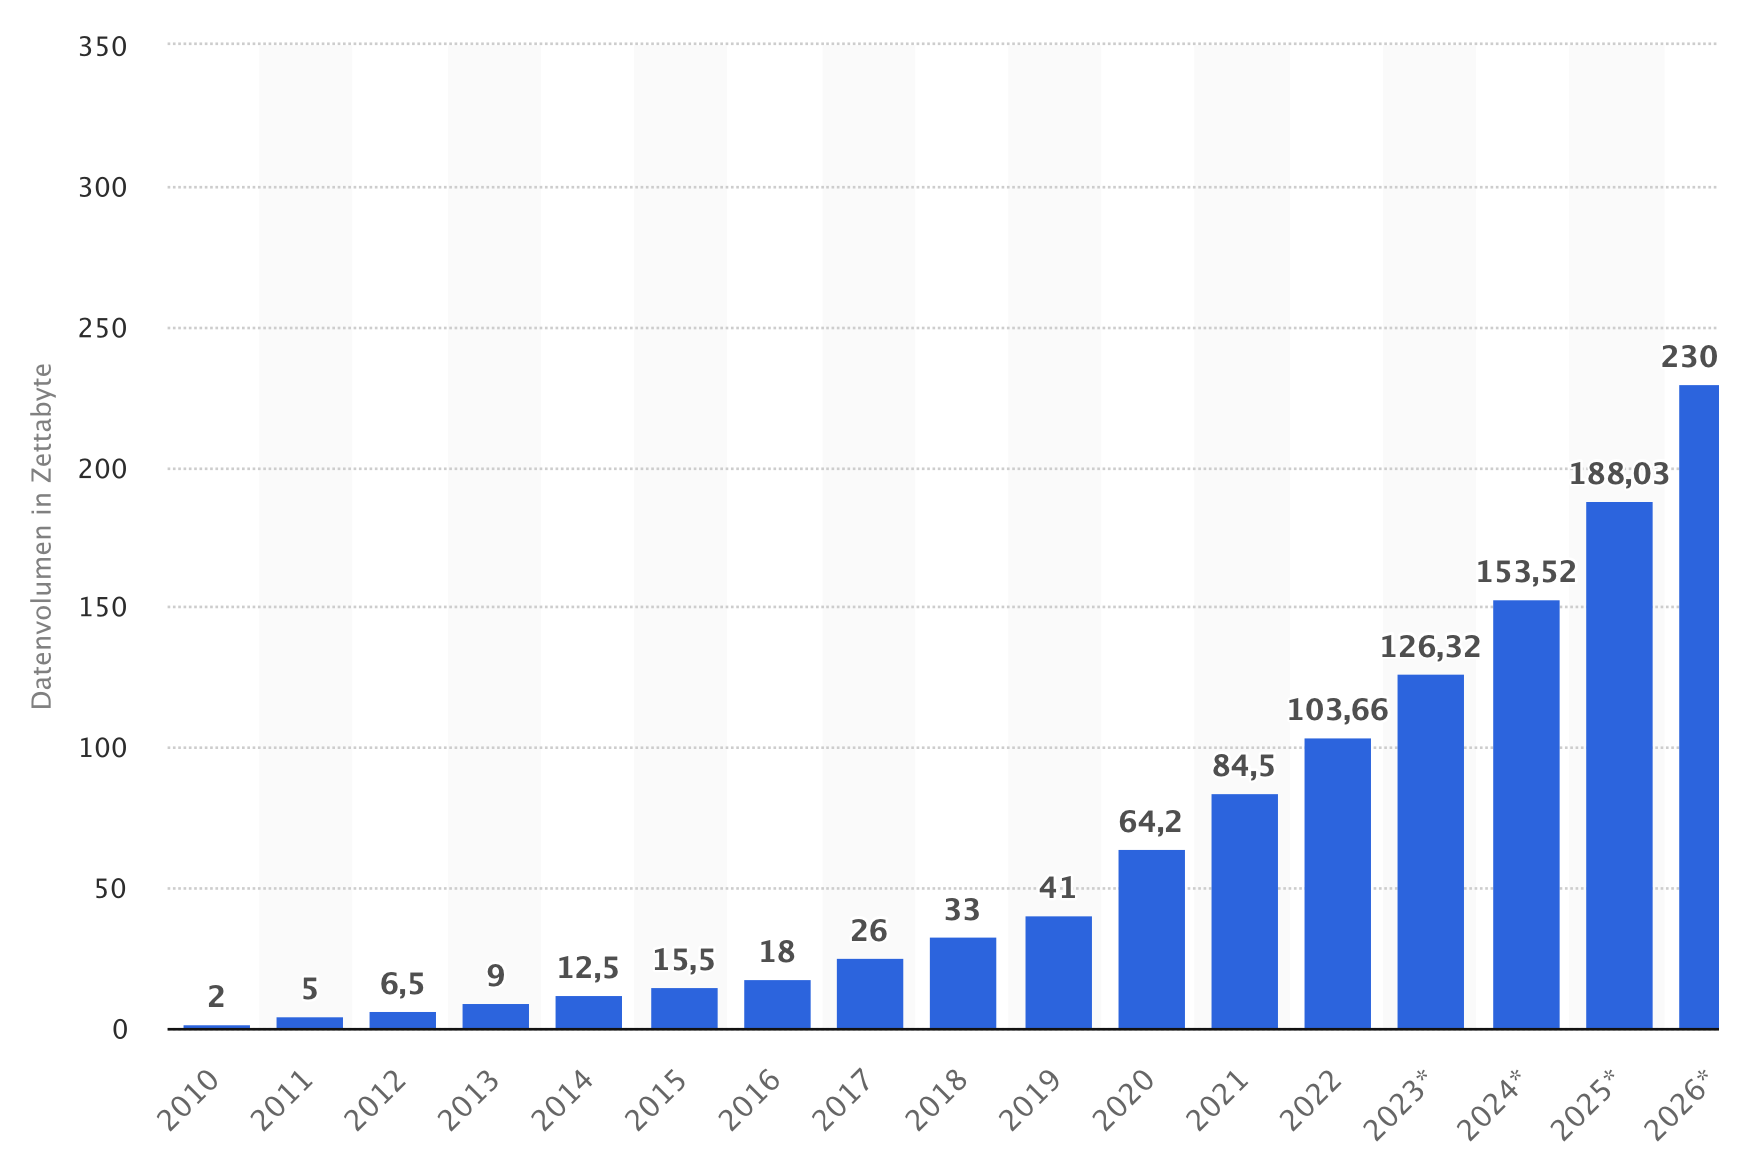
\includegraphics[width=0.48\textwidth]{DatenvolumenStatistik}
    \end{center}
    \vspace{-0.5cm}
    \caption{Volumen der weltweit generierten Daten bis 2027 \cite{Datenmengen}}
    \label{fig:DatenvolumenStatistik}
    \vspace{-0.5cm}
  \end{wrapfigure}
Weltweit wurden im Jahr 2022 Daten im Umfang von 103.66 Zettabyte erfasst \cite{Datenmengen}. Diese Zahl wird sich laut Statistik \ref{fig:DatenvolumenStatistik} bis zum Jahr 2026 verdoppelt haben. Angesicht dieser Zahlen, sind Datenbanken aus der heutigen Zeit nicht wegzudenken. Sie bieten eine Möglichkeit, große Mengen an Daten strukturiert abzuspeichern und anschließend auszuwerten.\\
Hierbei werden Datenbanken grundsätzlich in zwei Kategorien unterteilt. Relationale Datenbank und "Nicht relationale Datenbanken". Unterschiede der Datenbankarten machen sich in der Sprache zum Auswerten der DB, ihrer Skalierbarkeit, der Struktur, der Eigenschaften und der Unterstützung durch die Community bemerkbar. \cite{SQLNoSQL} 

\subsection{SQL - Structured Query Language}
\begin{wrapfigure}{r}{0.5\textwidth}
    \vspace{-1.2cm}
    \begin{center}
      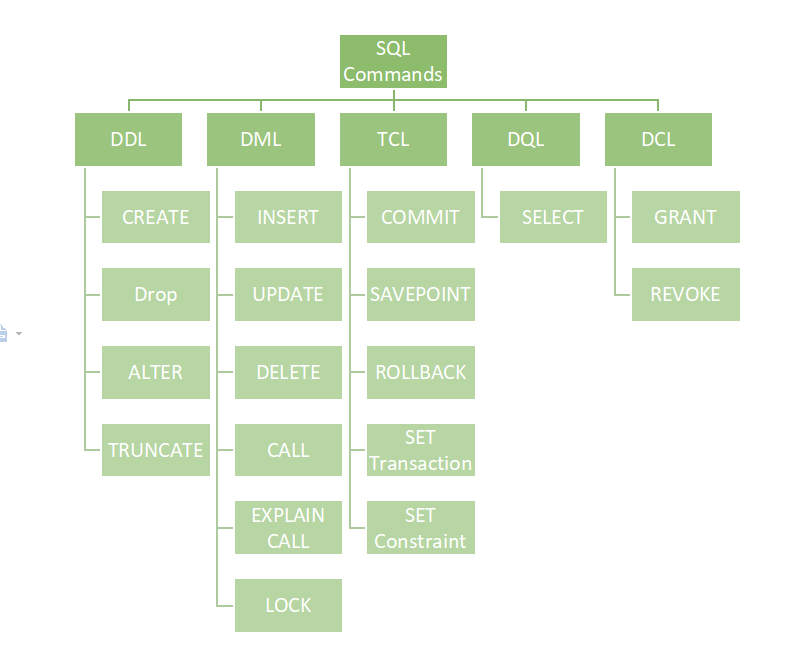
\includegraphics[width=0.48\textwidth]{SQLCommands}
    \end{center}
    \vspace{-0.5cm}
    \caption{SQL Befehls Kategorien \cite{SQLCommands}}
    \label{fig:SQLCommands}
    \vspace{-0.5cm}
  \end{wrapfigure}
IBM-Forscher Edgar F. Codd definierte 1969 ein Datenbankmodell für Relationale Datenbanken. Auf Grundlagen seiner Forschung begann, in den folgenden Jahren, die Entwicklung der Sprache \ac{sequel}. Codds Modell basiert auf der Zuordnung von Schlüsseln. Nach einigen Überarbeitungen der Implementierung wurde diese anschließend in \ac{sql} umbenannt.\cite{SQL}\\
\ac{sql} ermöglicht insbesondere die Speicherung, Bearbeitung so wie eine Abfrage von Daten in einer Datenbank. Mithilfe des Prinzips der Schlüssel können Datensätze miteinander verknüpft werden. Somit kann einem Benutzernamen beispielsweise ein echter Name, eine Telefonnummer und eine E-Mail Adresse zugewiesen werden.\cite{SQL}\\
Die besondere Eigenschaft von \ac{sql} ist das Konzept von Arrays. Relationale Datenbanken bestehen aus Arrays, welche sich mithilfe von verschiedenen Befehlen erzeugen und bearbeiten. \cite{SQL}\\
\ac{sql} bietet eine Reihe von Befehlen, welche die Interaktion mit der Datenbank ermöglichen. Diese können grundsätzlich in 5 Kategorien eingeteilt werden (siehe Abb. \ref{fig:SQLCommands}). Die wichtigsten Befehle sind dabei \textit{INSERT}, \textit{UPDATE} und \textit{DELEAT}, mit welchen sich Datensätze schreiben und bearbeiten lassen. Zudem der kommt der \textit{SELECT} Befehl, welcher das Auslesen von Datensätzen ermöglicht. Um die Tabellenstruktur der Datenbank zu bearbeiten kommen die Befehle \textit{CREATE} und \textit{DROP} zum Einsatz. \cite{SQLCommands}\\
Natürlich bietet die Programmiersprache eine weitaus komplexere Syntax, um Datensätze sortiert auswerten zu können. Eine vollständige Dokumentation der Sprache findet sich auf der w3school Webseite \cite{SQLDoku}.